\chapter{Temperatura a partir de la entropía y la energía}

\lectureoverview{La temperatura aparece primero como una conversión de las unidades de los termómetros humanos a unidades de energía microscópica. Tras realizar la conversión correspondiente de la entropía termodinámica a la entropía estadística adimensional, describimos el equilibrio mediante una familia uniparamétrica de distribuciones de probabilidad. La derivada \(dE/dS\) define entonces la temperatura, y las dos primeras leyes muestran por qué una diferencia de temperatura determina el sentido del flujo de energía.}

\section{Factores de conversión y unidades humanas}

Muchas constantes de la física son factores de conversión. La velocidad de la luz convierte una distancia en un tiempo:
\begin{equation}
 t=\frac{x}{c}.
\end{equation}
Si las distancias y los tiempos se miden en unidades compatibles, se puede fijar \(c=1\). No desaparece ningún efecto físico; simplemente se han expresado ambos tipos de medida en una escala común.

La constante de Boltzmann tiene el mismo carácter. Convierte la temperatura que indica un termómetro en una escala humana en energía. El adjetivo \emph{de escala humana} es importante. Estas unidades se eligen porque los instrumentos macroscópicos pueden producirlas y resolverlas, no porque la dinámica microscópica las distinga de manera especial.

El grado Celsius se fijó dividiendo en cien partes el intervalo entre los puntos de congelación y ebullición del agua a presión estándar. El kelvin usa un grado del mismo tamaño, pero sitúa el cero en el cero absoluto. Elegir otra sustancia, otro intervalo o grados Fahrenheit cambiaría los números, pero no la física.

\begin{classroomqa}
\audiencequestion{¿La escala Fahrenheit ya se había creado en el siglo XVII?}
\lecturerresponse{Aquí no hace falta precisar la fecha. Lo importante es que todas esas escalas se diseñaron en torno a temperaturas que las personas podían alcanzar y medir. El tamaño de sus grados es convencional, no microscópico.
\lecturetimestamp{00:01:34--00:01:50}}
\end{classroomqa}

Cuando se crearon estas escalas, el origen molecular del calor aún no estaba al alcance de la experimentación. Un termómetro macroscópico podía detectar un cambio de un grado, mientras que no se podía medir la energía de una sola molécula. Por eso era natural inventar una unidad de temperatura antes de saber que, en el fondo, la temperatura es una escala de energía.

\section{Por qué la temperatura tiene unidades de energía}

Consideremos un gas monoatómico diluido. Que sea diluido significa que, para lo que nos interesa ahora, podemos despreciar las energías de interacción entre moléculas. En equilibrio térmico, la equipartición asigna \(T_{\mathrm K}/2\) veces la constante de Boltzmann a cada grado de libertad traslacional cuadrático. En tres dimensiones espaciales,
\begin{equation}
 \left\langle E_{\mathrm{kin}}\right\rangle
 =\frac{3}{2}k_{\mathrm B}T_{\mathrm K}.
 \label{eq:sm2-equipartition-kelvin}
\end{equation}
El factor tres cuenta el movimiento en las direcciones \(x\), \(y\) y \(z\). El factor un medio procede de la energía cinética cuadrática.

Esta relación no es exclusiva de una especie molecular. En una mezcla de helio y oxígeno en equilibrio, todas las partículas con traslación libre tienen la misma energía cinética media del centro de masas, aunque las partículas más pesadas se muevan más despacio. Como
\begin{equation}
 E_{\mathrm{kin}}=\frac{1}{2}mv^2,
\end{equation}
a igual energía característica le corresponde \(v\propto m^{-1/2}\).

La misma idea puede llevarse a un ejemplo deliberadamente extremo. Suspendamos una bola de bolos en un fluido y dejemos que el sistema completo alcance el equilibrio. Sus grados de libertad traslacionales brownianos están regidos por la misma escala de energía que los de una molécula. La velocidad de la bola es extraordinariamente menor porque su masa es extraordinariamente mayor, pero la temperatura compara escalas de energía, no velocidades.

A temperatura ambiente, \(T_{\mathrm K}\) es aproximadamente \(300\,\mathrm K\), mientras que la energía de un grado de libertad microscópico es ínfima en julios. Por consiguiente, el factor de conversión es muy pequeño:
\begin{equation}
 k_{\mathrm B}\simeq 1.38\times10^{-23}\,
 \mathrm{J\,K^{-1}}.
 \label{eq:sm2-boltzmann-value}
\end{equation}
Su escala y el número de Avogadro están relacionados; no es una coincidencia:
\begin{equation}
 R=N_{\mathrm A}k_{\mathrm B}.
\end{equation}
La constante de los gases \(R\) describe un mol, mientras que \(k_{\mathrm B}\) describe la escala correspondiente por constituyente microscópico.

La combinación \(k_{\mathrm B}T_{\mathrm K}\) aparece una y otra vez en las fórmulas fundamentales. Por eso es más sencillo definir
\begin{equation}
 T\equiv k_{\mathrm B}T_{\mathrm K}.
 \label{eq:sm2-energy-temperature}
\end{equation}
A partir de ahora \(T\) tiene unidades de energía, y \eqref{eq:sm2-equipartition-kelvin} pasa a ser
\begin{equation}
 \left\langle E_{\mathrm{kin}}\right\rangle=\frac{3}{2}T.
 \label{eq:sm2-equipartition-natural}
\end{equation}
Si la energía se mide en julios, la temperatura se mide en julios. Si la energía se mide en electronvoltios, la temperatura se mide en electronvoltios. No existe ninguna nueva unidad natural llamada unidad de temperatura.

\section{Dos convenciones para la entropía}

La misma conversión aparece en el caso de la entropía. La termodinámica macroscópica surgió del análisis de las máquinas térmicas. Carnot aportó el razonamiento decisivo sobre las máquinas; más tarde, Clausius introdujo la entropía termodinámica y el símbolo \(S\). En la notación que usaremos aquí, llamemos \(S_{\mathrm C}\) a esa magnitud macroscópica. Sus unidades son energía dividida por temperatura indicada por un termómetro, por ejemplo, julios por kelvin.

La entropía estadística es adimensional. Para una distribución discreta,
\begin{equation}
 S=-\sum_i p_i\log p_i.
 \label{eq:sm2-statistical-entropy}
\end{equation}
Con logaritmos naturales, una alternativa binaria equiprobable tiene entropía \(\log2\); con logaritmos en base dos, esa misma cantidad se denomina un bit. Las dos convenciones para la entropía están relacionadas por
\begin{equation}
 S=\frac{S_{\mathrm C}}{k_{\mathrm B}},
 \qquad
 S_{\mathrm C}=k_{\mathrm B}S.
 \label{eq:sm2-entropy-conversion}
\end{equation}
Un valor macroscópico moderado en \(\mathrm{J\,K^{-1}}\) corresponde a una entropía adimensional enorme, porque cuenta información distribuida entre un número enorme de constituyentes microscópicos.

Las ecuaciones \eqref{eq:sm2-energy-temperature} y \eqref{eq:sm2-entropy-conversion} establecen la convención que usaremos en todo el texto:
\[
 [T]=[\text{energy}],
 \qquad
 [S]=1.
\]
La constante de Boltzmann puede desaparecer ahora de las fórmulas de trabajo. Siempre se puede reintroducir reemplazando \(T\) por \(k_{\mathrm B}T_{\mathrm K}\) y \(S\) por \(S_{\mathrm C}/k_{\mathrm B}\).

\begin{classroomqa}
\audiencequestion{Aparte del factor \(3/2\), ¿la nueva temperatura es simplemente una energía medida en julios?}
\lecturerresponse{Sí, si se eligen los julios como unidad de energía. El julio es la unidad MKS \(\mathrm{kg\,m^2\,s^{-2}}\). También se podrían usar electronvoltios o cualquier otra unidad de energía; en tal caso, la temperatura tendría que expresarse en esa misma unidad. El factor \(3/2\) corresponde al ejemplo del gas ideal, no a la definición de temperatura.
\lecturetimestamp{00:15:49--00:16:45}}
\end{classroomqa}

\begin{classroomqa}
\audiencequestion{Si el pizarrón especifica kelvin, ¿no es entonces \(k_{\mathrm B}\) una constante definida?}
\lecturerresponse{Queda definida una vez especificadas tanto la unidad de temperatura como la de energía. Si se cambia el kelvin por grados Fahrenheit, o los julios por electronvoltios, cambia su valor numérico. Esa dependencia de las unidades es precisamente la que caracteriza a un factor de conversión.
\lecturetimestamp{00:16:46--00:18:33}}
\end{classroomqa}

\begin{classroomqa}
\audiencequestion{¿Se determina experimentalmente el valor numérico de la constante de Boltzmann?}
\lecturerresponse{Sí. Históricamente, para evaluarla se necesitaba información microscópica sobre los átomos y su densidad numérica. Boltzmann entendió la relación entre la energía molecular y la temperatura antes de que esas magnitudes se conocieran con precisión, de manera parecida a como Newton conocía el papel de la constante gravitatoria antes de que se midiera con exactitud.
\lecturetimestamp{00:18:46--00:20:00}}
\end{classroomqa}

\section{El equilibrio es un estado estadístico}

La conversión de unidades todavía no ha definido la temperatura. Tocar algo caliente ofrece una intuición biológica útil, pero la temperatura es una magnitud física derivada, construida a partir de la energía y la entropía.

Imaginemos un sistema en contacto con un entorno grande cuyas condiciones macroscópicas se mantienen fijas. Puede intercambiar energía con él. Si al principio el sistema tiene demasiada energía, en promedio la pierde; si tiene muy poca, en promedio la gana. En equilibrio térmico siguen produciéndose intercambios microscópicos, pero el flujo neto medio en cualquiera de los dos sentidos es nulo.

Sea \(i\) la etiqueta de un estado microscópico exacto del sistema, y sea \(E_i\) la energía de ese estado. El equilibrio no significa que el sistema quede inmóvil en un único estado. La interacción con el entorno cambia continuamente el microestado, así que asignamos una probabilidad \(P_i\) a cada posibilidad. Las relaciones básicas son
\begin{align}
 \sum_i P_i &=1,
 \label{eq:sm2-normalization}\\
 \sum_i P_iE_i &=\overline E,
 \label{eq:sm2-mean-energy}\\
 S&=-\sum_iP_i\log P_i.
 \label{eq:sm2-equilibrium-entropy}
\end{align}
La barra sobre \(\overline E\) destaca que la energía del subsistema fluctúa. Una medición puede dar un valor y la siguiente, otro; al repetir las mediciones, se obtiene la distribución cuya media es \eqref{eq:sm2-mean-energy}.

\begin{figure}[t]
\centering
\includegraphics[width=0.82\textwidth]{lecture_02_figure_02.png}
\caption{Normalización y energía media en el pizarrón: \(\sum_iP(i)=1\) y \(\sum_iP(i)E(i)=\langle E\rangle\).}
\lectureframe{00:24:10}
\end{figure}

\section{Una familia parametrizada por la energía media}

La distribución de equilibrio depende mucho de la energía media. Si ponemos una olla de agua al fuego, \(\overline E\) aumenta; si la dejamos en la nieve, \(\overline E\) disminuye. Las probabilidades cambian con ella. Por tanto, el equilibrio debe entenderse no como una sola distribución, sino como una familia uniparamétrica:
\begin{equation}
 P_i(\overline E).
 \label{eq:sm2-family}
\end{equation}
Cada miembro satisface
\begin{align}
 \sum_iP_i(\overline E)&=1,
 \label{eq:sm2-family-normalization}\\
 \sum_iP_i(\overline E)E_i&=\overline E.
 \label{eq:sm2-family-mean}
\end{align}

\begin{figure}[t]
\centering
\includegraphics[width=0.88\textwidth]{lecture_02_figure_03.png}
\caption{La transición a \(P(i,\overline E)\). Las ecuaciones anteriores de normalización, energía media y entropía permanecen visibles mientras se introduce la familia de distribuciones.}
\lectureframe{00:26:29}
\end{figure}

Para un gráfico esquemático, ordenemos los estados según el valor creciente de \(E_i\). Así, el eje horizontal puede leerse como el índice \(i\) o como la energía correspondiente. Una energía media mayor desplaza el peso de probabilidad hacia los estados situados más a la derecha. El área total bajo cada curva debe ser igual a uno.

\begin{figure}[t]
\centering
\includegraphics[width=0.88\textwidth]{lecture_02_figure_04.png}
\caption{Varias distribuciones esquemáticas \(P(i,\overline E)\). Las curvas con más peso hacia la derecha tienen mayor energía media, y todas están normalizadas.}
\lectureframe{00:28:40}
\end{figure}

\begin{figure}[t]
\centering
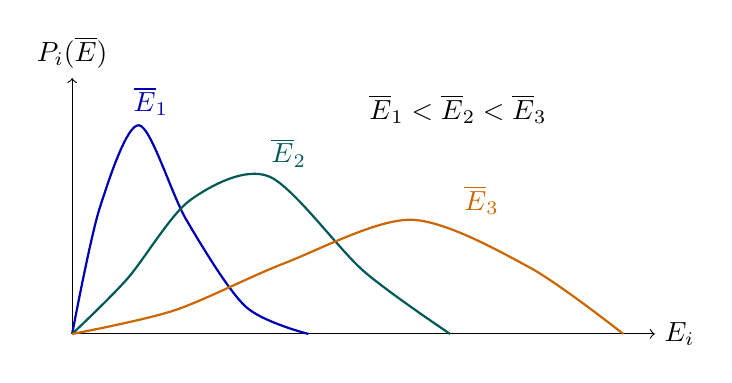
\begin{tikzpicture}[x=1cm,y=1cm]
\draw[->] (0,0) -- (7.4,0) node[right] {$E_i$};
\draw[->] (0,0) -- (0,3.25) node[above] {$P_i(\overline E)$};
\draw[thick,blue!70!black]
  plot[smooth] coordinates {(0,0) (0.35,1.6) (0.85,2.65) (1.45,1.45)
  (2.2,0.35) (3.0,0)};
\draw[thick,teal!70!black]
  plot[smooth] coordinates {(0,0) (0.7,0.7) (1.5,1.7) (2.5,2.0)
  (3.7,0.8) (4.8,0)};
\draw[thick,orange!80!black]
  plot[smooth] coordinates {(0,0) (1.3,0.3) (2.7,0.9) (4.3,1.45)
  (5.8,0.85) (7.0,0)};
\node[blue!70!black] at (1.0,2.95) {\(\overline E_1\)};
\node[teal!70!black] at (2.75,2.3) {\(\overline E_2\)};
\node[orange!80!black] at (5.2,1.7) {\(\overline E_3\)};
\node at (4.9,2.85) {\(\overline E_1<\overline E_2<\overline E_3\)};
\end{tikzpicture}
\caption{Una versión limpia del esquema del pizarrón. No hace falta que las curvas tengan estas formas precisas; solo se usan la normalización y el orden de sus energías medias.}
\end{figure}

\begin{classroomqa}
\audiencequestion{¿Es circular esta notación? La energía media se calcula a partir de la distribución, pero la distribución está parametrizada por la energía media.}
\lecturerresponse{Partamos de una familia uniparamétrica de distribuciones de equilibrio elegida empíricamente. Cada miembro tiene una energía media. Si miembros distintos tienen medias distintas, se puede usar esa media como parámetro para nombrar la familia. La notación todavía no deriva la familia; más adelante, la distribución de Boltzmann proporcionará esa derivación.
\lecturetimestamp{00:28:35--00:29:44}}
\end{classroomqa}

\begin{classroomqa}
\audiencequestion{¿Por qué se habla de energía media y no de energía total?}
\lecturerresponse{El subsistema intercambia energía con un baño térmico, como la atmósfera que rodea un recipiente de gas cuyas paredes dejan pasar el calor. Su energía instantánea fluctúa. Al hacer muchas mediciones se obtiene una distribución, y \(\overline E\) es la media de esos resultados. La energía del sistema cerrado más grande, formado por el subsistema y el baño, sí puede mantenerse fija.
\lecturetimestamp{00:29:46--00:30:56}}
\end{classroomqa}

\begin{classroomqa}
\audiencequestion{¿Pueden tener la misma energía distintos estados microscópicos? ¿Y pueden tener la misma energía media distintas distribuciones?}
\lecturerresponse{Ambas cosas son posibles. La condición sobre la energía media, por sí sola, permite muchas distribuciones, así que hace falta otro argumento físico para obtener la familia uniparamétrica especial de equilibrio. Más adelante se derivarán su origen y su forma de Boltzmann. Que distintos microestados tengan la misma energía es otra cuestión, denominada degeneración.
\lecturetimestamp{00:30:58--00:32:22}}
\end{classroomqa}

\subsection{Etiquetas de estado, degeneración y correlación}

Hay que mantener separados varios conceptos que se confunden con facilidad.

Primero, muchas distribuciones de probabilidad pueden tener la misma energía media. La familia uniparamétrica de equilibrio no se obtiene únicamente de la condición sobre la energía media. Es la familia particular que selecciona la equilibración; más adelante veremos que su forma es la distribución de Boltzmann.

Segundo, varios microestados distintos pueden tener la misma energía. Esto se llama degeneración. En el análisis del pizarrón, por el momento se ignoran las degeneraciones exactas para poder ordenar los estados sin ambigüedad según su energía. De hecho, la degeneración es común cuando un sistema tiene simetrías, pero no plantea ningún problema conceptual: se conserva la etiqueta del estado \(i\), se permiten valores repetidos de \(E_i\) y se suman todos los estados.

Tercero, correlación no es otra manera de decir degeneración. La correlación concierne a una distribución conjunta de dos magnitudes aleatorias y pregunta si conocer una modifica las probabilidades de la otra. Las etiquetas mutuamente excluyentes \(i\) y \(j\) en una lista de microestados no son, por sí solas, dos variables aleatorias cuya correlación se esté calculando.

\begin{classroomqa}
\audiencequestion{¿La construcción supone que los distintos estados \(i\) son independientes? ¿Y qué ocurre si dos de ellos están correlacionados?}
\lecturerresponse{Una etiqueta de estado es un valor posible de una sola variable aleatoria microscópica. La independencia y la correlación requieren dos variables con una distribución conjunta, así que esos términos no se aplican directamente a dos etiquetas alternativas de esta lista. Que distintos estados tengan la misma energía es, en cambio, una cuestión de degeneración.
\lecturetimestamp{00:32:23--00:33:22}}
\end{classroomqa}

\begin{classroomqa}
\audiencequestion{¿Qué ocurre si dos estados distintos tienen exactamente la misma energía?}
\lecturerresponse{Eso es degeneración. Para el gráfico inmediato adoptamos la simplificación de suponer que no coinciden dos energías y ordenamos los estados por energía creciente. Las fórmulas de probabilidad que obtendremos más adelante no requieren esta suposición; los estados degenerados simplemente se cuentan por separado.
\lecturetimestamp{00:33:23--00:34:04}}
\end{classroomqa}

\begin{classroomqa}
\audiencequestion{¿Es arbitrario el significado del índice \(i\)?}
\lecturerresponse{Los estados microscópicos en sí no son arbitrarios: cada uno especifica todas las posiciones, los momentos u otros datos necesarios para una descripción exacta. Sus nombres sí son arbitrarios, así que para la figura elegimos etiquetas en orden creciente de energía.
\lecturetimestamp{00:34:06--00:35:15}}
\end{classroomqa}

\section{La entropía pasa a ser una función de la energía}

Cada miembro de la familia de equilibrio tiene una entropía. Al sustituir \eqref{eq:sm2-family} en \eqref{eq:sm2-equilibrium-entropy} se obtiene
\begin{equation}
 S(\overline E)
 =-\sum_iP_i(\overline E)\log P_i(\overline E).
 \label{eq:sm2-entropy-energy}
\end{equation}
No se trata de una función universal común a todos los sistemas físicos. Depende del espectro del sistema y de su familia de equilibrio. Sin embargo, una vez especificada esa familia, la energía y la entropía quedan vinculadas: al recorrerla, ambas cambian.

En los sistemas ordinarios, la probabilidad suele repartirse entre más estados a medida que aumenta la energía media; por eso, \(S\) suele aumentar con \(\overline E\). Por ahora suponemos que esta relación es suave e invertible localmente. Las excepciones son importantes, pero el caso sencillo permite presentar la definición que necesitamos.

\section{La derivada que define la temperatura}

Planteemos una pregunta concreta: ¿cuánto debe cambiar la energía media para aumentar la entropía en una alternativa binaria? En unidades de logaritmo natural, ese incremento de entropía es \(\log2\).

Para miembros cercanos de una familia suave,
\begin{equation}
 dE=\frac{dE}{dS}\,dS.
 \label{eq:sm2-differential-identity}
\end{equation}
Por ahora, la ecuación no es más que la regla de la cadena. Sin embargo, su coeficiente tiene exactamente las dimensiones y el papel físico que se necesitan para la temperatura.

\begin{definition}La temperatura en unidades de energía es
\begin{equation}
 T\equiv\frac{dE}{dS}.
 \label{eq:sm2-temperature-definition}
\end{equation}
De forma equivalente,
\begin{equation}
 dE=T\,dS,
 \qquad
 dS=\frac{1}{T}\,dE.
 \label{eq:sm2-fundamental-differentials}
\end{equation}
\end{definition}

Para un cambio suficientemente pequeño de un bit,
\begin{equation}
 \Delta E\simeq T\log2.
 \label{eq:sm2-one-bit-energy}
\end{equation}
La elección de un bit solo sirve para hacer tangible la derivada. La misma relación local se cumple para cualquier cambio pequeño de entropía.

\begin{classroomqa}
\audiencequestion{Si la entropía se escribió como \(S(E)\), ¿no sería más natural usar la derivada \(dS/dE\)?}
\lecturerresponse{Si la relación es invertible localmente, cualquiera de las dos derivadas contiene la misma información:
\[
 \frac{dE}{dS}=\left(\frac{dS}{dE}\right)^{-1}.
\]
Por convención, la temperatura es \(dE/dS\), mientras que la temperatura inversa es \(dS/dE=1/T\).
\lecturetimestamp{00:40:24--00:40:54}}
\end{classroomqa}

Aquí solo cambia una variable termodinámica, así que bastan las derivadas ordinarias. Cuando se permite que cambien el volumen, el número de partículas, la magnetización u otras variables, hay que usar derivadas parciales e indicar qué magnitudes se mantienen fijas. La definición actual es el corte unidimensional de esa geometría termodinámica más general.

\subsection{Por qué se cancela la constante de Boltzmann}

Volvamos brevemente a las unidades de los termómetros. Usando
\[
 T=k_{\mathrm B}T_{\mathrm K},
 \qquad
 S=\frac{S_{\mathrm C}}{k_{\mathrm B}},
\]
la relación fundamental se convierte en
\begin{align}
 dE
 &=\bigl(k_{\mathrm B}T_{\mathrm K}\bigr)
   d\left(\frac{S_{\mathrm C}}{k_{\mathrm B}}\right)\\
 &=T_{\mathrm K}\,dS_{\mathrm C}.
 \label{eq:sm2-carnot-form}
\end{align}
La temperatura aporta un factor de \(k_{\mathrm B}\) y la entropía, el factor recíproco. Se cancelan. Por eso un texto convencional de termodinámica puede escribir \eqref{eq:sm2-carnot-form} sin mostrar la constante de Boltzmann.

\begin{classroomqa}
\audiencequestion{¿Tiene que ser invertible \(S(E)\)?}
\lecturerresponse{No siempre. En los sistemas ordinarios y el régimen que consideramos aquí, al aumentar la energía suele ensancharse la distribución de equilibrio y aumentar la entropía, de modo que \(S(E)\) es monótona y \(T>0\). Los sistemas con espectros acotados pueden ser contraejemplos, incluidos los regímenes en que la entropía disminuye al aumentar la energía y la temperatura estadística es negativa. Por ahora dejaremos esos casos de lado.
\lecturetimestamp{00:44:30--00:45:57}}
\end{classroomqa}

\section{De la derivada abstracta a lo caliente y lo frío}

La definición mediante una derivada es universal, pero sigue siendo abstracta. Queremos recuperar la afirmación familiar de que la energía fluye de un cuerpo más caliente a otro más frío. El dolor que produce tocar una superficie caliente es una respuesta biológica; el color y la radiación emitida dependen de las propiedades de la luz. Una definición estadística también debe tener sentido para un gas idealizado, incluso cuando se ignora la radiación.

\begin{classroomqa}
\audiencequestion{¿Podría usarse la luz que emite un objeto caliente para definir la temperatura de forma fundamental?}
\lecturerresponse{La radiación es un termómetro útil, pero introduce la física de la luz. La mecánica estadística debe definir la temperatura para sistemas como una caja de gas sin depender de sus propiedades ópticas. El sentido del intercambio de energía es el criterio más general.
\lecturetimestamp{00:46:42--00:47:20}}
\end{classroomqa}

Preparemos dos sistemas \(A\) y \(B\), cada uno inicialmente en equilibrio por separado, con temperaturas \(T_A\) y \(T_B\). Al principio están aislados uno del otro. Después los conectamos mediante un contacto térmico débil: el \emph{tubo delgado} permite que pasen pequeñas cantidades de energía en ambos sentidos sin destruir la identidad de ninguno de los dos subsistemas.

\begin{figure}[t]
\centering
\includegraphics[width=0.88\textwidth]{lecture_02_figure_05.png}
\caption{Los sistemas \(A\) y \(B\), preparados por separado y caracterizados por las temperaturas \(T_A\) y \(T_B\), justo antes de considerar el contacto térmico débil.}
\lectureframe{00:48:55}
\end{figure}

\begin{figure}[t]
\centering
\begin{tikzpicture}[>=Stealth]
\draw[rounded corners,thick,fill=blue!6] (0,0) rectangle (2.6,2.4);
\draw[rounded corners,thick,fill=orange!8] (5.4,0) rectangle (8,2.4);
\draw[thick] (2.6,1.35) -- (5.4,1.35);
\draw[thick] (2.6,1.05) -- (5.4,1.05);
\draw[<->,very thick] (3.15,1.2) -- (4.85,1.2)
  node[midway,above] {\(\delta E\)};
\node at (1.3,1.45) {\Large \(A\)};
\node at (6.7,1.45) {\Large \(B\)};
\node at (1.3,0.65) {\(T_A,S_A,E_A\)};
\node at (6.7,0.65) {\(T_B,S_B,E_B\)};
\node at (4,0.35) {\small weak thermal contact};
\end{tikzpicture}
\caption{La energía fluctúa a través del contacto débil mientras el sistema combinado permanece aislado.}
\end{figure}

Supongamos, sin pérdida de generalidad, que
\begin{equation}
 T_B>T_A.
 \label{eq:sm2-temperature-order}
\end{equation}
La experiencia indica que \(B\) debería perder energía y \(A\) debería ganarla. Tres hechos convierten esa expectativa en un cálculo.

\subsection{Aditividad de la entropía}

Para dos subsistemas débilmente acoplados, cuyas alternativas microscópicas se combinan de forma independiente, el número de posibilidades conjuntas es el producto de los números de posibilidades de cada uno:
\[
 W_{AB}=W_AW_B.
\]
La entropía es logarítmica, así que
\begin{equation}
 S_{\mathrm{tot}}=S_A+S_B.
 \label{eq:sm2-entropy-additivity}
\end{equation}
Se obtiene el mismo resultado directamente a partir de la entropía de Shannon de una distribución producto.

\begin{classroomqa}
\classquestion{¿Por qué se suman las entropías de los sistemas combinados?}
\lecturerresponse{Porque se multiplica el número de alternativas subyacentes y la entropía toma un logaritmo:
\(\log(W_AW_B)=\log W_A+\log W_B\). La interacción débil es lo que permite describir los subsistemas y obtener esta forma aditiva dominante.
\lecturetimestamp{00:51:06--00:52:03}}
\end{classroomqa}

\subsection{La primera y la segunda ley}

El sistema combinado está aislado, por lo que la energía intercambiada internamente se conserva:
\begin{equation}
 dE_A+dE_B=0,
 \qquad
 dE_B=-dE_A.
 \label{eq:sm2-first-law}
\end{equation}
Esta es la primera ley en el experimento que estamos considerando.

Tomamos aquí la segunda ley como un postulado cuya fundamentación más profunda explicaremos más adelante. A medida que los sistemas conectados se relajan hacia su nuevo equilibrio,
\begin{equation}
 dS_{\mathrm{tot}}=dS_A+dS_B\geq0.
 \label{eq:sm2-second-law}
\end{equation}
La desigualdad estricta describe la relajación espontánea que los aleja del equilibrio; en el equilibrio se cumple la igualdad para la variación reversible de primer orden.

Por último, la definición de temperatura se aplica a cada subsistema:
\begin{equation}
 dE_A=T_A\,dS_A,
 \qquad
 dE_B=T_B\,dS_B.
 \label{eq:sm2-two-temperatures}
\end{equation}

\begin{figure}[H]
\centering
\includegraphics[width=0.88\textwidth]{lecture_02_figure_06.png}
\caption{Las relaciones de los dos subsistemas \(dE_A=T_A\,dS_A\) y \(dE_B=T_B\,dS_B\) al concluir el argumento en el pizarrón.}
\lectureframe{00:54:00}
\end{figure}

\subsection{El signo del flujo de energía}

Estas ecuaciones ya determinan el sentido de la transferencia neta. Sustituyamos \(dS_A=dE_A/T_A\), \(dS_B=dE_B/T_B\) y \eqref{eq:sm2-first-law} en \eqref{eq:sm2-second-law}:
\begin{align}
 dS_{\mathrm{tot}}
 &=\frac{dE_A}{T_A}+\frac{dE_B}{T_B}\\
 &=dE_A\left(\frac{1}{T_A}-\frac{1}{T_B}\right)\geq0.
 \label{eq:sm2-flow-sign}
\end{align}
Si \(T_B>T_A>0\), entonces
\[
 \frac{1}{T_A}-\frac{1}{T_B}>0.
\]
Por tanto, la ecuación \eqref{eq:sm2-flow-sign} exige que
\[
 dE_A>0,
 \qquad
 dE_B<0.
\]
El sistema más frío \(A\) gana energía y el más caliente \(B\) la pierde. Cuando \(T_A=T_B\), el cambio de entropía de primer orden no favorece ningún sentido, y los intercambios microscópicos se equilibran, de modo que el flujo neto es nulo. Así, la derivada abstracta \(T=dE/dS\) reproduce la distinción operativa entre lo caliente y lo frío.
